\documentclass[12pt,a4paper]{article}
\usepackage[top=25.4mm, bottom=25.4mm, left=19.1mm, right=19.1mm]{geometry}


\usepackage[latin2]{inputenc}
\usepackage{graphicx}
\graphicspath{ {./images/} }
\usepackage{ulem}
\usepackage{enumitem}
\usepackage{amsmath}
\usepackage[document]{ragged2e}

\setlength{\parindent}{4em}
\setlength{\parskip}{1em}
\usepackage{hyperref}

\usepackage{fancyhdr}
\pagestyle{fancy}
\fancyhf{}
\fancyhead[LO]{\textbf{\small IoT and Smart Analytics}\\
\text{\small A Program by IIITH and TalentSprint}}

\usepackage{xcolor}
\usepackage{lipsum}

\rhead{\begin{picture}(0,0) \put(-250,-2){
\includegraphics[width=9cm]{EXP_06_Images/ts-iisc-logo-pr.png}} \end{picture}}
\cfoot{\thepage}


\begin{document}

\begin{center}
\textbf{\large \\EXPERIMENT 00 }\\[6pt]
TinkerCAD Prototyping of Electronic Circuits, Using Multimeter, Breadboard and Soldering technique
\end{center}

\textbf{\large LEARNING OBJECTIVES:}\\[3pt]
At the end of this experiment, participants will be able to:\vspace{-6mm}\begin{enumerate}
 \setlength\itemsep{-0.3em}
\item Prototype basic electronic components/circuits with TinkerCAD
\item Use and understand multimeter with its functionalities
\item Use and understand breadboard and its connections
\item Know how to measure current, voltage, resistance, and continuity testing with a multimeter
\item Know Soldering techniques 
\end{enumerate}

\textbf{\large APPARATUS REQUIRED:}\\
\vspace{-3mm}
\begin{enumerate}
 \setlength\itemsep{-0.3em}
\item A good Internet connection
\item Digital Multimeter
\item Breadboard
\item Power Adapter
\item DC-DC Voltage Converter Power Supply Module
\item LED - 1pcs
\item Resistor 1k$\Omega$ - 1pcs
\item Jumper Wires
\item Soldering Iron, Stand and Wire, and Flux
\item 4x6 Cm Printed Circuit Board
\end{enumerate}

\begin{justify}
\textbf{\large THEORY}\\[3pt]
\textbf{A)	Digital Multimeter}: A digital Multimeter is a test tool used to measure two or more electrical values-principally voltage (volts), current (amps), and resistance (ohms). It is a standard diagnostic tool for technicians in the electrical/electronic industries.\par
\noindent Digital Multimeter (DMM) combines the testing capabilities of single-task meters-the Voltmeter (for measuring volts), Ammeter (amps), and Ohmmeter (ohms). Often, they include several additional specialized features or advanced options. Technicians with specific needs, therefore, can seek out a model targeted to meet their needs. Fig. 1 shows a Multimeter with labeled components.\par
\noindent Three red circled holes are the input jacks where leads are inserted. Two out of them are positive and negative for connecting with corresponding DC polarity. The face of a Digital Multimeter typically includes four components as given below:

\begin{center} 
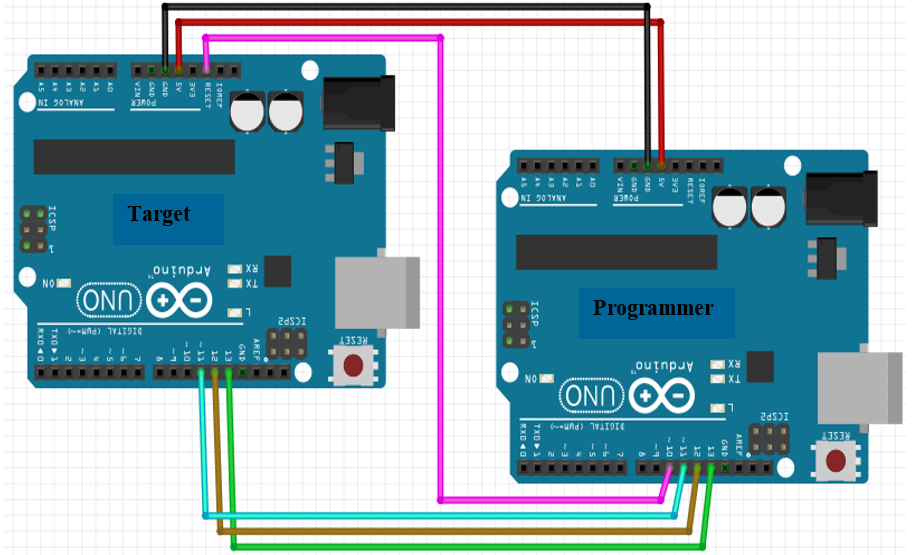
\includegraphics[scale=0.7]{EXP_00_Images/fig1.png}
\end{center}
\vspace{-10mm}
\begin{center} {Figure 1. DMM with labelled components [1]}\end{center}

\begin{itemize}
\setlength\itemsep{-0.3em}
\item Display: Where measurement readouts can be viewed.
\item Buttons: For selecting various functions, the options vary by model.
\item Dial (or rotary switch): Select primary measurement values (volts, amps, ohms).
\item Input jacks: Where test leads are inserted
\end{itemize}

\noindent Test leads are flexible, insulated wires (red for positive, black for negative) that plug into the DMM. They serve as the conductor from the item being tested to the multimeter. The probe tips on each lead are used for testing circuits. Table 1 below gives the DMM functions and symbol description.
\vspace{-6mm}
\begin{center} {Table 1. DMM functions and symbols description}\end{center}
\vspace{-10mm}
\begin{center} 
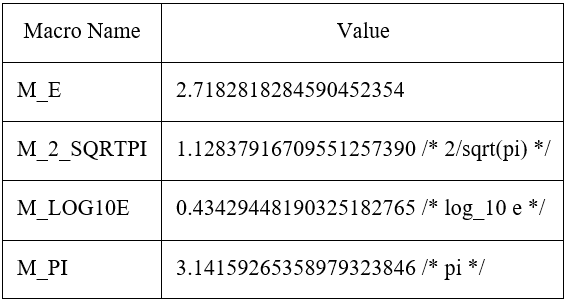
\includegraphics[scale=1]{EXP_00_Images/table1.png}
\end{center}


\noindent \textbf{B) Breadboard}A breadboard is a solderless device for a quick prototype with electronics and test circuit designs. Most electronic components in electronic circuits can be interconnected by inserting their leads or terminals into the holes and then making connections through wires where appropriate. The breadboard has strips of metal underneath the board and connects the holes on the top of the board.


\begin{center} 
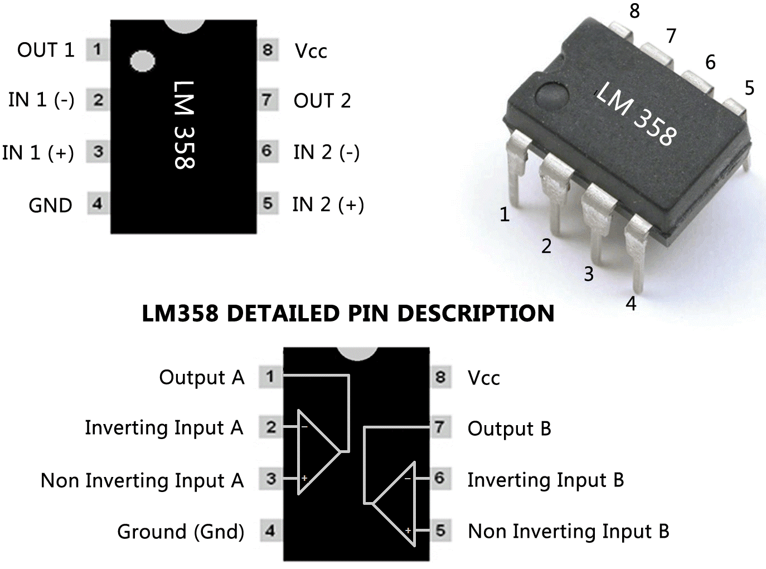
\includegraphics[scale=0.65]{EXP_00_Images/fig2.png}
\end{center}
\vspace{-10mm}
\begin{center} {(A) Breadboard section with metallic strip underneath [2]   (B)  Separated metallic strip [3]}\end{center}
\vspace{-10mm}
\begin{center} {Figure 2. Breadboard connections underneath}\end{center}


\noindent The vertical columns of the breadboard are called terminals, while the long horizontal rows are called power rails because they are "usually" used to connect the power supply to the breadboard. The breadboard has strips of metal underneath the board and connects the holes on the top of the board. The metal strips are laid out as shown in fig. 2. Note that the top and bottom rows of holes are connected horizontally and split in the middle while the remaining holes are connected vertically.\par
\noindent Note that exact configurations might vary from breadboard to breadboard. For example, some breadboards have the buses broken in half along the length of the breadboard (useful if we need to supply the circuit with two different voltage levels, see fig. 3).\par
\noindent Note how all holes in the selected row are connected, so as in the holes in the selected column. To interconnect the selected row (node A) and column (node B), a cable going from any hole in the row to any hole in the column is needed, as shown in fig. 3.\par
\vspace{-7mm}
\begin{center} 
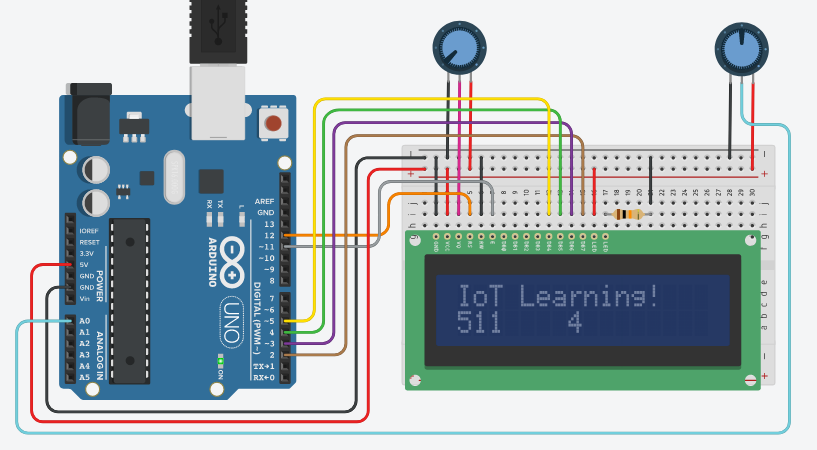
\includegraphics[scale=0.8]{EXP_00_Images/fig3.png}
\end{center}
\vspace{-8mm}
\begin{center} {Figure 3. Breadboard horizontal/vertical nodes and making a connection [4]}\end{center}

\noindent For example, consider making a simple LED circuit on the breadboard as given in fig. 4. Note the difference between the correct and incorrect connections in fig. 5. In the correct version, the two legs are on different columns (nodes); in the incorrect version, the two legs are connected to the same column (node), which is equivalent to shorting or tie together the two legs of the LED.\par
\noindent As shown in fig. 6, the LED has two legs. The longer leg (anode) is connected to the VCC (+Ve terminal) of the power supply (node N1), while the smaller leg (cathode) is connected to one end of the resistor (node N2). The other end of the resistor is connected to GROUND (-Ve terminal) (node N3). The LED is a polarized device, which means it matters how it is connected while the resistor is not polarized so that pins can be inverted with no effect on the circuit's behavior. 


\begin{center} 
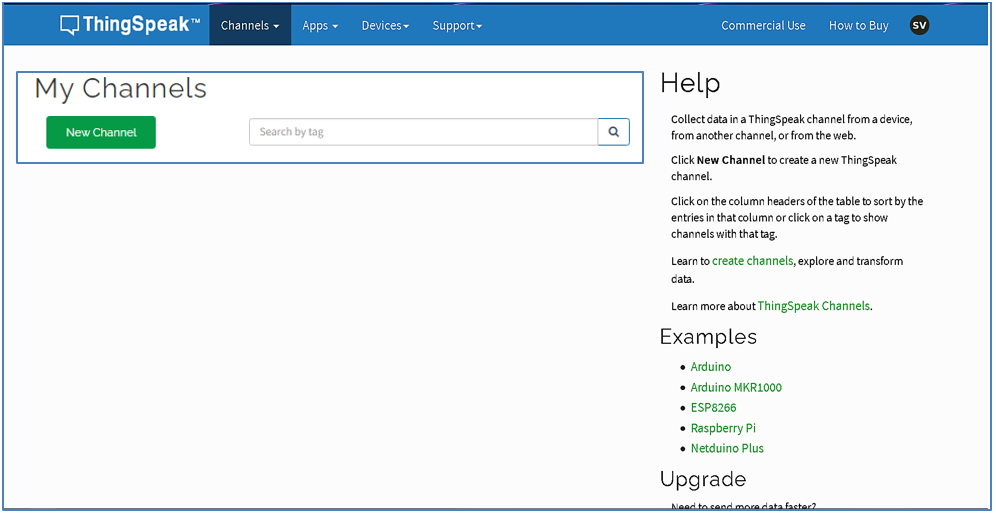
\includegraphics[scale=0.45]{EXP_00_Images/fig4.png}
\end{center}
\vspace{-8mm}
\begin{center} {Figure 4. LED circuit to implement on breadboard}\end{center}


\begin{center} 
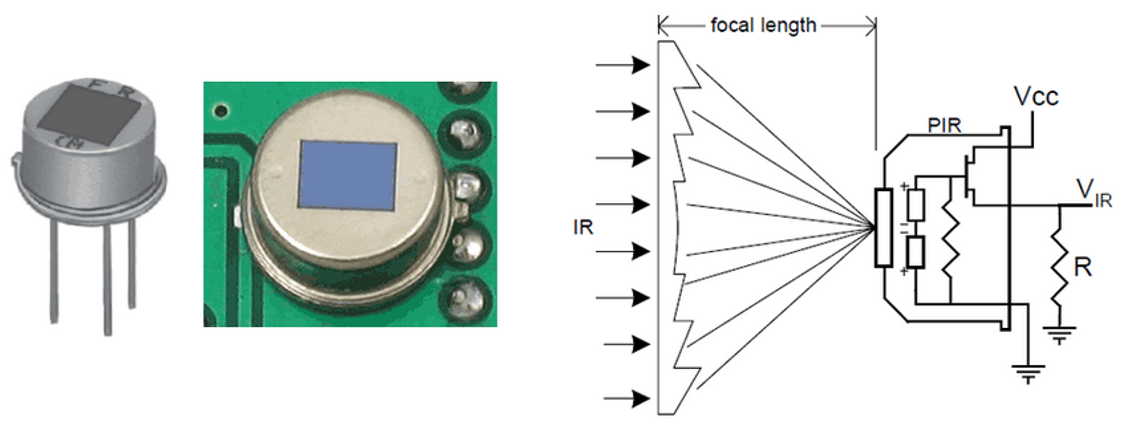
\includegraphics[scale=0.5]{EXP_00_Images/fig5.png}
\end{center}
\vspace{-8mm}
\begin{center} {Figure 5. Correct and incorrect LED connection on breadboard [5]}\end{center}

\begin{center} 
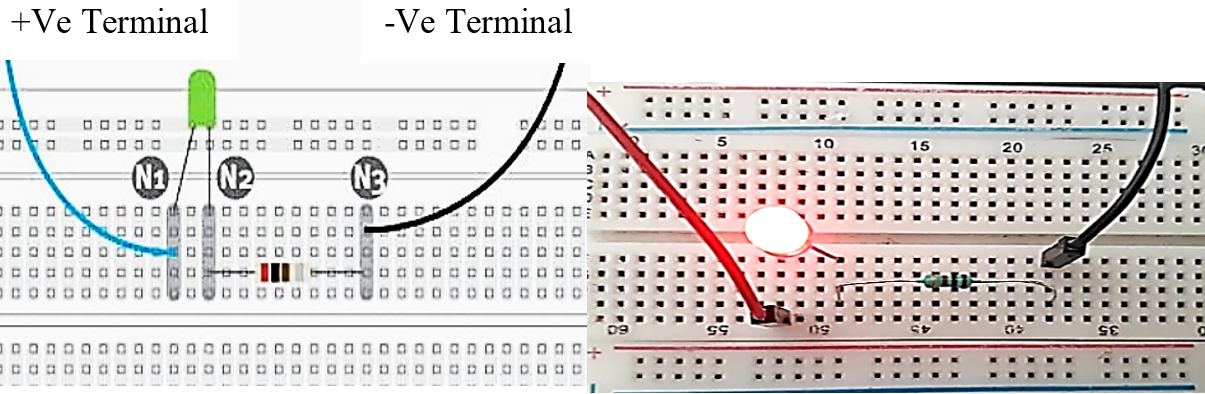
\includegraphics[scale=0.4]{EXP_00_Images/fig6.png}
\end{center}
\vspace{-8mm}
\begin{center} {Figure 6. Physical realization of LED circuit on breadboard }\end{center}



\noindent \textbf{\large PROCEDURE}\\[6pt]
\textbf{1)	Making a simple circuit with an LED and Measuring Current/Voltage}\\
\textbf{A)TinkerCAD}\\[6pt]
\noindent TinkerCAD is a free online service for creating basic 3D shapes and developing digital prototypes of electronic components. These prototypes include basic circuits with LEDs, bussers, switches, and even sensors. 
The process used in TinkerCAD is often used for rapid prototyping. Prototyping is a process where we can develop electronic circuits in a flexible manner that can be quickly updated and modified to test various options when developing a project or a product. We will use this process of prototyping to learn how to create basic electronic circuits. The software helps create Arduino projects virtually without any need for physical hardware and allows easy simulation of circuits online.\\[6pt]
\noindent \textbf{Creating a TinkerCAD account:}
\vspace{-5mm}
\begin{enumerate}
 \setlength\itemsep{-0.3em}
\item Open \href{https://www.tinkercad.com/}{TinkerCAD} on the browser.
\item  Click 'Join Now' on the right top of the screen and create an account in TinkerCAD with your email ids. Or sign in with Google at your convenience.
\item  A successful login will transition to a dashboard with the user name, as shown in fig. 7 above, providing options for designing 3D models, circuits, code blocks, etc., on the left of the screen.
\item Click on circuits to seamlessly enjoy building circuits. Happy tinkering!!
\end{enumerate}

\vspace{-5mm}
\noindent \textbf{Building circuits with TinkerCAD }
\vspace{-5mm}
\begin{enumerate}
\setlength\itemsep{-0.3em}
\item Click on 'Create New Circuit' and save the design by providing a file name on the left top of the screen..
\item  The screen would look as in fig. 8 given below, after completing all the steps here.

\begin{center} 
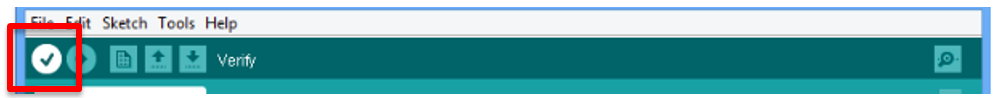
\includegraphics[scale=0.45]{EXP_00_Images/fig7.png}
\end{center}
\vspace{-8mm}
\begin{center} {Figure 7. Dashboard of TinkerCAD }\end{center}

\begin{center} 

\includegraphics[scale=0.88]{EXP_00_Images/fig8.png}
\end{center}
\vspace{-8mm}
\begin{center} {Figure 8. Workspace of TinkerCAD circuits }\end{center}

\item A circuit generally consists of input and output components and a processing device. Search for the required components and drag all of them onto the workspace. We can click on one point of a component and drag it to another point (of a component or a breadboard point) to give a wire connection. Also, note that we can give different colors and labels.
\item After the circuit is done, click on 'Code' and selects 'Text.' Write the code here. Note: The serial monitor is also available below. Click on the serial monitor to access it to either provide inputs to the circuit or to read the output. A Serial monitor is a window that allows the user to send messages from the PC to Arduino and to receive messages from the Arduino (Arduino will be introduced later).
\item Now click on 'Start Simulation' to view the results. Click on 'Stop Simulation' to stop the simulation. Note: The user cannot change the positions of components or make any changes in the circuit while the simulation is on. Stop the simulation from making any changes in the circuit.
\item All the designs will be saved in the dashboard. We can reopen them and tinker with the designs again.\par

\noindent A detailed process of how to build circuits using TinkerCAD is explained below by using an LED. Here we will build a simple circuit using an LED, a 1kΩ resistor (We can use a resistor of our choice), and power it with a 5V power source. After that, we will measure the voltage drop across the components and the current flowing through the circuit. The schematic of the circuit is shown in fig. 9, which we are going to implement.

\end{enumerate}

\begin{center} 
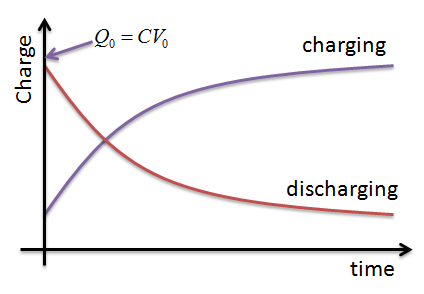
\includegraphics[scale=0.5]{EXP_00_Images/fig9.png}
\end{center}
\vspace{-8mm}
\begin{center} {Figure 9. Circuit diagram for TinkerCAD [6] }\end{center}


\noindent The stepwise process is given below:
\vspace{-3mm}
\begin{enumerate}[label={(\alph*)}]

\item Select a power source by writing 'power supply' on the search bar and drag it onto the workspace. Clicking on it results in a dialog box, where we can put voltage as 5V.

 \begin{center} 
 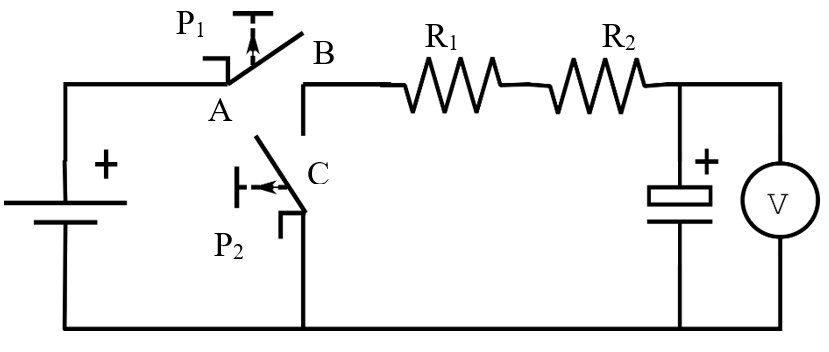
\includegraphics[scale=0.5]{EXP_00_Images/fig10.png}
 \end{center}
 \vspace{-8mm}
 \begin{center} {Figure 10. Selecting power source}\end{center}

 \item Search for all other required components (i.e., LED and a 1k$\Omega$ resistor, Bread Board) and drag all of them onto the workspace. Note: We can press 'R' or click on the button on the top left to rotate a component to a required angle. See fig. 11.

 \begin{center} 
 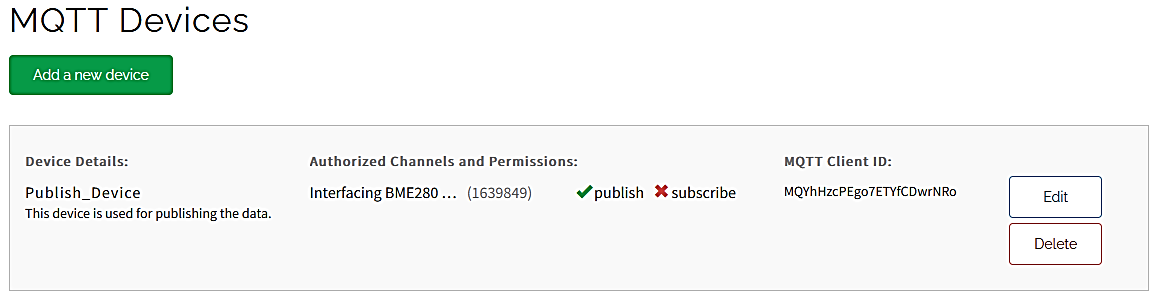
\includegraphics[scale=0.6]{EXP_00_Images/fig11.png}
 \end{center}
 \vspace{-8mm}
 \begin{center} {Figure 11. Dragging all other components}\end{center}



 \item Now we can click on one point of a component and drag to another point (of a component or a breadboard point) to give a wire connection. Also, note that we can give different colors and labels. Make all the required connections by wiring up the components as in the schematic shown in fig. 12 below. Make sure we are connecting with proper terminals. We can hover on the terminals of the components (in TinkerCAD) to check if they are positive or negative. This circuit turns the LED ON when the simulation is started.

 \begin{center} 
 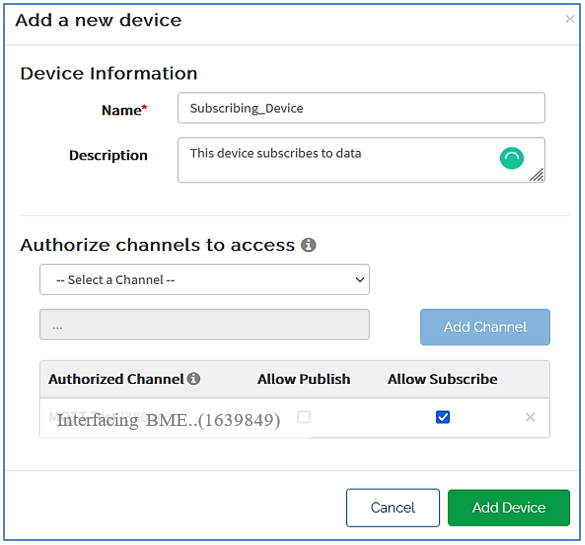
\includegraphics[scale=1]{EXP_00_Images/fig12.png}
 \end{center}
 \vspace{-8mm}
 \begin{center} {Figure 12. Connecting the components \& simulation}\end{center}
 \end{enumerate}


 \noindent \textbf{Measuring Voltage \& Current:} We now will use the Multimeter available in TinkerCAD to measure voltage, current across the LED, and the voltage across the resistor. The process is similar to the actual hardware implementation. However, care must be taken while using the probes for the actual hardware implementation. Make sure that the probes are in contact with appropriate terminals and polarity.

 \begin{enumerate}
 \item Search for a Multimeter in the components list. This Multimeter can operate as a Voltmeter, Ammeter, and Ohmmeter by choosing the appropriate mode required. A dialog box, as in fig. 13, appears after clicking on the Multimeter.

\begin{center} 
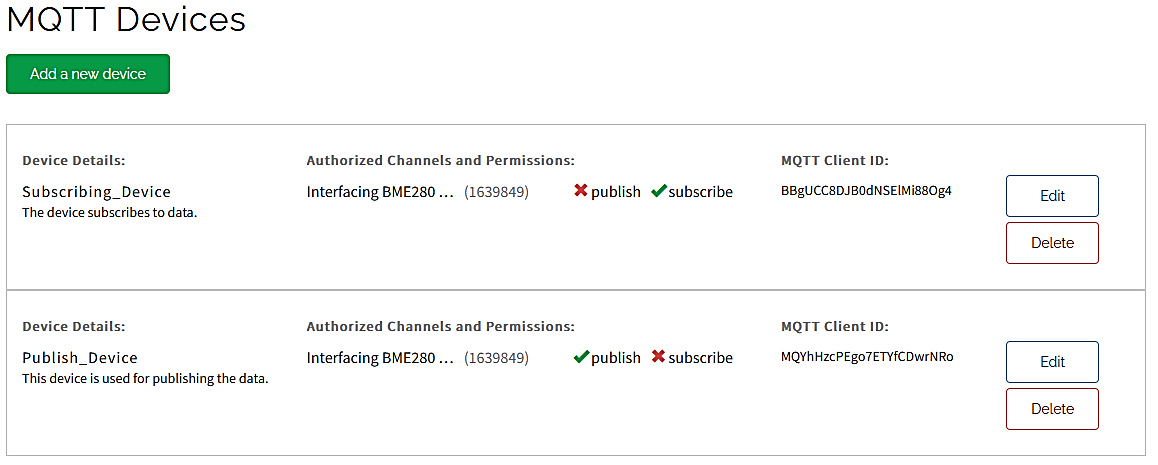
\includegraphics[scale=1.3]{EXP_00_Images/fig13.png}
\end{center}
\vspace{-8mm}
\begin{center} {Figure 13. Selecting Voltage mode}\end{center}

\item To measure the voltage across the LED, choose the Multimeter in voltage mode and connect it parallel to the LED, as shown in fig. 14. Ensure that the Voltmeter is connected parallel to the component across which voltage has to be measured as they have extremely high internal resistance. This is required so that any current flowing in the circuit is not diverted into the Voltmeter.

\begin{center} 
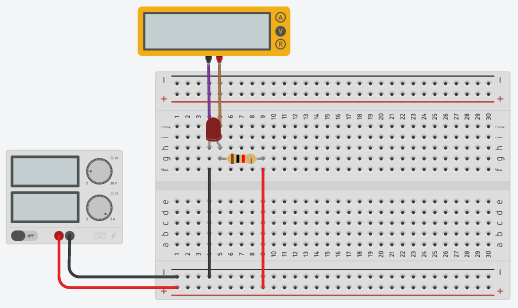
\includegraphics[scale=1]{EXP_00_Images/fig14.png}
\end{center}
\vspace{-8mm}
\begin{center} {Figure 14. Voltmeter connected in parallel to the LED}\end{center}

\item Click on 'Start Simulation.' We can see the voltage as measured by the Multimeter in fig. 15. It shows the voltage drop across the LED as measured by the Voltmeter when a 1k$\Omega$ resistor is used.\\[6pt]
Once the battery is connected to the LED, the circuit is closed, and charges (here electrons) start flowing from the negative terminal of the power source to the positive terminal.

\begin{center} 
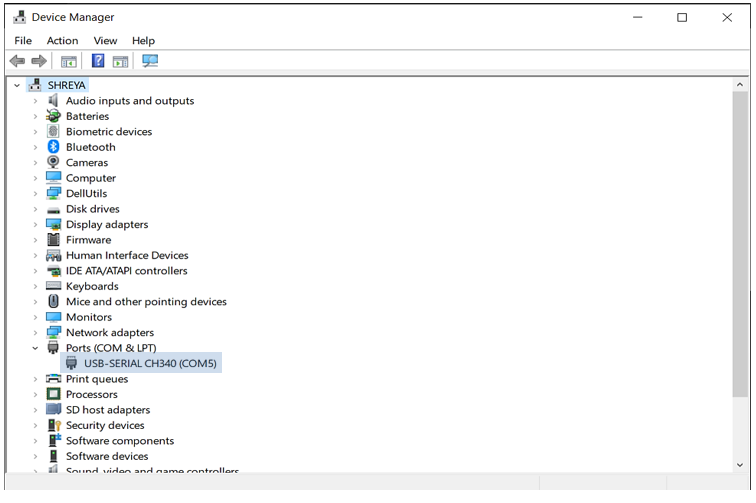
\includegraphics[scale=1]{EXP_00_Images/fig15.png}
\end{center}
\vspace{-8mm}
\begin{center} {Figure 15. Voltage reading after start of the simulation}\end{center}

In our circuit, the potential difference across the battery (terminals of the power supply) is 5V to 0V, 5V at negative and positive terminals, respectively. As the current flows and the circuit encounter, some resistance and some potentials are lost, voltage drops across that component. For example, a voltage drop can be observed in fig.16 across the resistor, and the LED as both offer resistance to the circuit.\par
Make sure we are connecting the LED using proper resistance. If a very small value is given, there is a possibility of a short circuit and the LED burns. We can check by decreasing the resistance up to 10$\Omega$, and the LED will burn.

\item The voltage drop across any component can be measured using a Voltmeter by connecting the multimeter in the voltage mode across the component. Figure 16 below shows the voltage drop across both the LED and the resistor after the simulation is started.

\begin{center} 
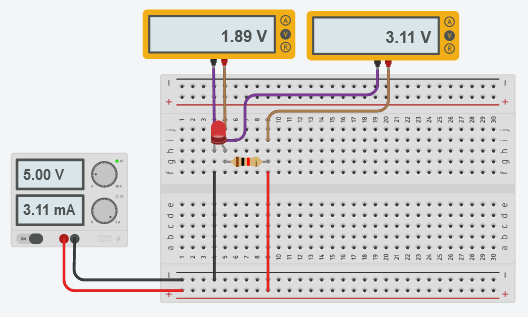
\includegraphics[scale=0.8]{EXP_00_Images/fig16.png}
\end{center}
\vspace{-8mm}
\begin{center} {Figure 16. Voltages across both LED and Resistor}\end{center}


\item To measure the current flowing through the circuit, the Multimeter has to be connected in the Amperage mode, and after simulation, we get the result as shown in fig. 17. The Multimeter must be connected in series with the component as the Multimeter has very low internal resistance. This arrangement is required because the total current flowing through the circuit should also flow through the Ammeter to measure its value.   

\begin{center} 
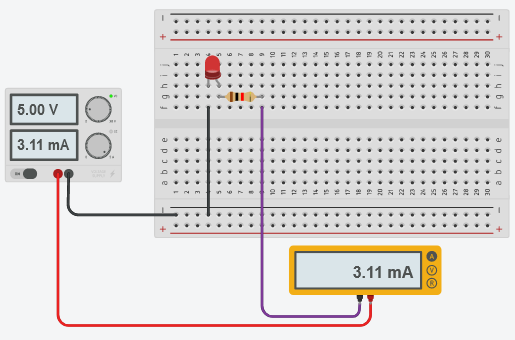
\includegraphics[scale=0.8]{EXP_00_Images/fig17.png}
\end{center}
\vspace{-8mm}
\begin{center} {Figure 17. Current measurement through the circuit}\end{center}


\item The resistance values can be changed, and different values of current and voltage drops can be observed for the corresponding resistances.
\item Both Voltmeter and Ammeter can be connected in a single circuit, as shown in fig. 18. Make sure the Voltmeter (Multimeter in 'Voltage' mode) is connected parallel to the components across which voltage drop must be measured, and Ammeter (Multimeter in 'Amperage' mode) is connected in series with the components through which the current flowing has to be measured.

\begin{center} 
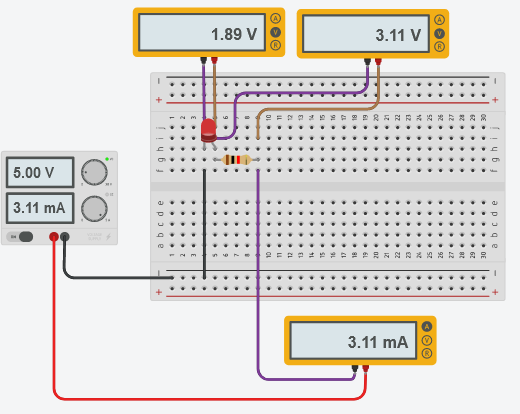
\includegraphics[scale=0.7]{EXP_00_Images/fig18.png}
\end{center}
\vspace{-8mm}
\begin{center} {Figure 18. Measuring both current and voltage}\end{center}

\item The Multimeter can be used in 'Resistance' mode to operate as an Ohmmeter, as given in fig. 19. Note: Ensure that the power supply is disconnected from the circuit while measuring the actual resistance of the component.
\begin{center} 
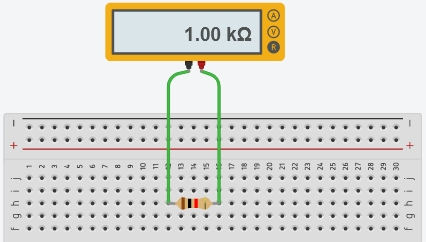
\includegraphics[scale=0.8]{EXP_00_Images/fig19.png}
\end{center}
\vspace{-8mm}
\begin{center} {Figure 19. Resistance measurement}\end{center}

\textbf{Note:} After changing the circuit, we must start the simulation every time to get the results.

\end{enumerate}

\noindent \textbf{B) Physical Realization: }\\[6pt]
\noindent We are going to use the following components as tabulated below from the apparatus.
\vspace{-3mm}
\begin{center} {Table 2.Figures of apparatus required.}\end{center}
\vspace{-8mm}
\begin{center} 
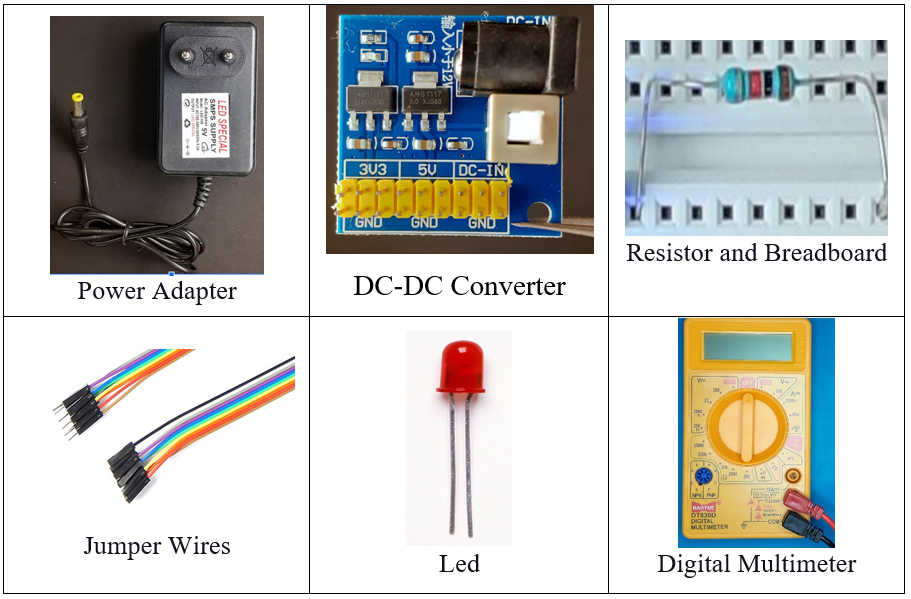
\includegraphics[scale=0.7]{EXP_00_Images/table2.png}
\end{center}

\noindent \textbf{Measuring Voltage }\\[3pt]
\noindent Hardware Setup: Connect the circuit as given in fig. 20 \& fig. 21. Connect the longer lead of the LED (called the anode) with one end of the resistor and then another end of the resistor to the 5V of DC power supply (DC to DC converter). Connect the shorter lead of the LED (called the cathode) to the ground of the DC to DC converter. Connect the power adapter to the AC mains and output end of the power adapter to the DC to DC converter. Duly check the connections and polarity of the LED. Switch on the AC mains, the LED of DC to DC Converter should glow and then push the button on DC to DC convertor, externally connected LED through resistor should glow. For basics on LED, you may want to go through this video \href{https://www.youtube.com/watch?v=Yo6JI_bzUzo}{link}. 

\begin{center} 
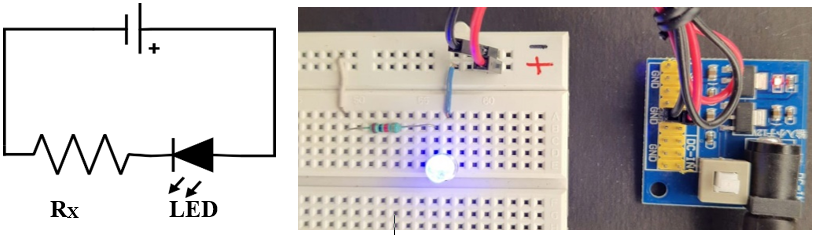
\includegraphics[scale=0.6]{EXP_00_Images/fig20_21.png}
\end{center}
\vspace{-8mm}
\begin{center} {Figure 20. Circuit Diagram \hspace{5mm} Figure 21. Circuit connection: LED with power supply}\end{center}
\vspace{-5mm}
\noindent Now follow the steps given below to measure voltage and current.\\
 \vspace{-10mm}
\begin{itemize}
 \setlength\itemsep{-0.3em}
\item Set the mode to 'V~' to measure AC voltage or to the 'V-' to measure DC voltage. In fig.22, the central knob of the multimeter is kept at DC voltage mode of operation.
\item Ensure the red probe is connected to the port with a V next to it.
\item Connect the red probe to the positive side of the component (i.e., the anode of the LED), where the current is coming. For the sake of simplicity, the resistor is not shown.
\item Connect the COM probe to the other side of the component.
\item Read the value on the display. Similarly, the voltage across the resistor can be measured.
\end{itemize}

\begin{center} 
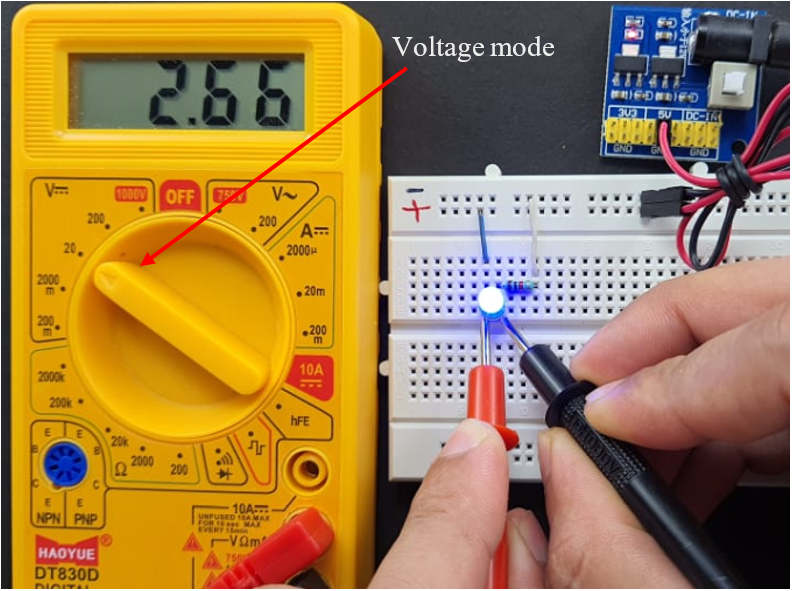
\includegraphics[scale=0.5]{EXP_00_Images/fig22.png}
\end{center}
\vspace{-8mm}
\begin{center} {Figure 22. Voltage measurement across LED}\end{center}

\noindent \textbf{Measuring current}
\vspace{-4mm}
\begin{itemize}
\setlength\itemsep{-0.3em}
\item Before measuring the current, ensure that the red probe is plugged in the right port.
\item Set the mode to A. We need to bear in mind that components in series share a current. So, we must connect the multimeter in series with the circuit. To place the multimeter in series, we need to place the red probe on the lead of a component and the black probe on the next component lead, as in fig.23, maintaining the polarity. 
\item The multimeter acts as if it was a wire in the circuit. If we disconnect the multimeter, the circuit won't work.
\item Read the value on the display.
\end{itemize}

\begin{center} 
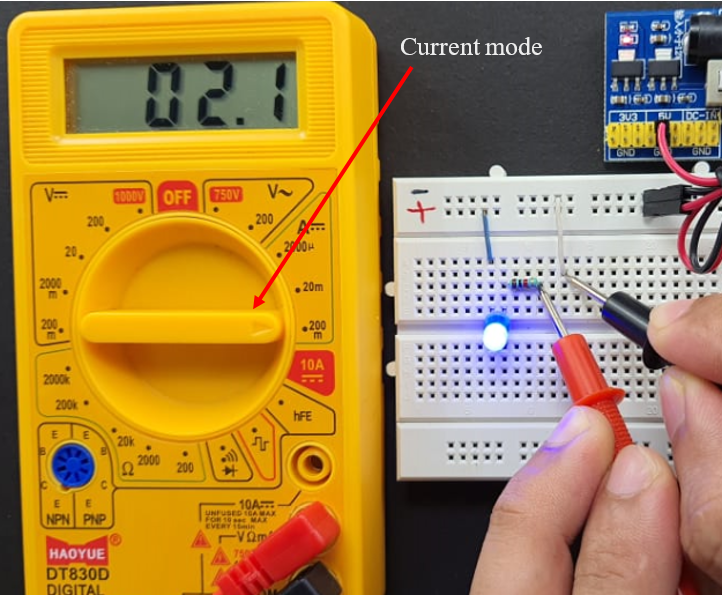
\includegraphics[scale=0.6]{EXP_00_Images/fig23.png}
\end{center}
\vspace{-8mm}
\begin{center} {Figure 23. Current measurement connections}\end{center}


\noindent \textbf{Measuring resistance}
\vspace{-4mm}
\begin{itemize}
 \setlength\itemsep{-0.3em}
\item Plug the red probe into the right port and turn the selection knob to the resistance section as given in fig. 24.
\item Connect the probes to the resistor leads. The way we connect the leads does not matter, and the result is the same.
\item Read the value on the display.
\end{itemize}

\begin{center} 
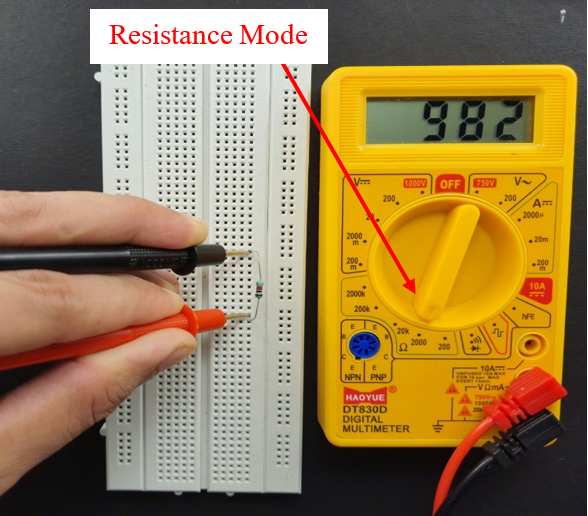
\includegraphics[scale=0.5]{EXP_00_Images/fig24.png}
\end{center}
\vspace{-8mm}
\begin{center} {Figure 24. Resistance measurement connections}\end{center}

\noindent \textbf{Checking continuity}
\vspace{-4mm}
\begin{itemize}
 \setlength\itemsep{-0.3em}
\item To use this functionality, select the mode that looks like a speaker. 
\item If there is very low resistance between two points, which is less than a few ohms, the two points are electrically connected, and we'll hear a continuous sound.
\item If the sound isn't continuous or there is no sound, then there is no connection between the two points.
\item The continuity check allows us to detect bugs such as faulty wires easily. It also helps us check if two points of the circuit are connected.
\item Touch the two probes together and, as they are connected, we'll hear a continuous sound. To test the continuity of a wire, we just need to connect each probe to the wire tips (See fig. 25)

\end{itemize}

\begin{center} 
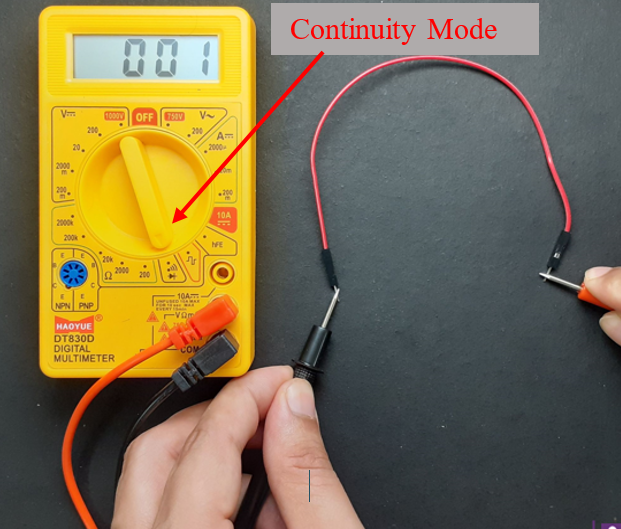
\includegraphics[scale=0.5]{EXP_00_Images/fig25.png}
\end{center}
\vspace{-8mm}
\begin{center} {Figure 25. Continuity checking}\end{center}
\vspace{3cm}
\noindent\textbf{2) Soldering Techniques}\\[3pt]
Table 3 shows the components from the apparatus list that are used for this experiment.
\vspace{-3mm}
\begin{center} {Table 3.Components used for Soldering Practice}\end{center}
\vspace{-10mm}
\begin{center} 
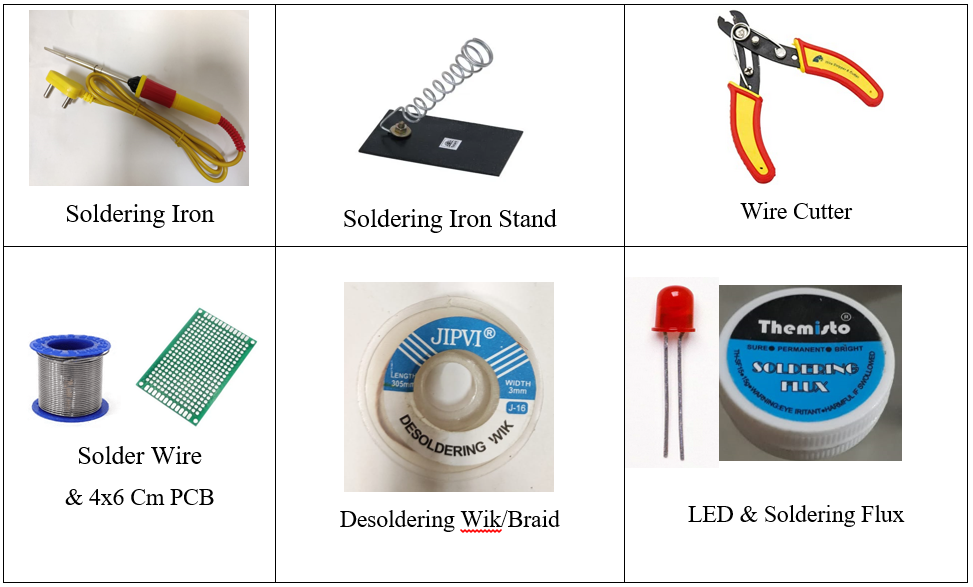
\includegraphics[scale=0.7]{EXP_00_Images/table3.png}
\end{center}

\noindent \textbf{A. \underline{Tinning The Tip}}\\[6pt]
\noindent Before we can start soldering, we need to prep the soldering iron by tinning the tip with the solder (covering the tip with a solder layer). This process will help improve the heat transfer from the iron to the item we're soldering. Tinning will also help to protect the tip and reduce wear.\\[5pt]
\textbf{Step 1:} Begin by making sure the tip is attached to the iron and screwed tightly in place. \\
\textbf{Step 2:} Turn on the soldering iron and let it heat up.\\
\textbf{Step 3:} Wipe the soldering iron tip on a damp, wet sponge or any wet cloth to clean it. Wait a few seconds to let the tip heat up again before proceeding to step 4. \\
\textbf{Step 4:} Hold the soldering iron in one hand and solder in the other. Touch the solder to the iron tip and make sure the solder flows evenly around the tip.\\
We should tin the tip of the iron before and after each soldering session to extend its life. Eventually, every tip will wear out and will need replacing when it becomes rough or pitted\\

\noindent  \textbf{B. \underline{How To Solder}}\\[6pt]
\noindent To better explain how to solder, we're going to demonstrate it with a real-world application. In this example, we're going to solder an LED to a circuit board.\\

\noindent \textbf{Step 1: Mount the Component :}  Begin by inserting the LED leads into the holes of the circuit board. Flip the board over and bend the leads outward at a 45 $^{\circ}$  angle. This process will help the component better connect with the copper pad and prevent it from falling out while soldering.


\begin{center} 
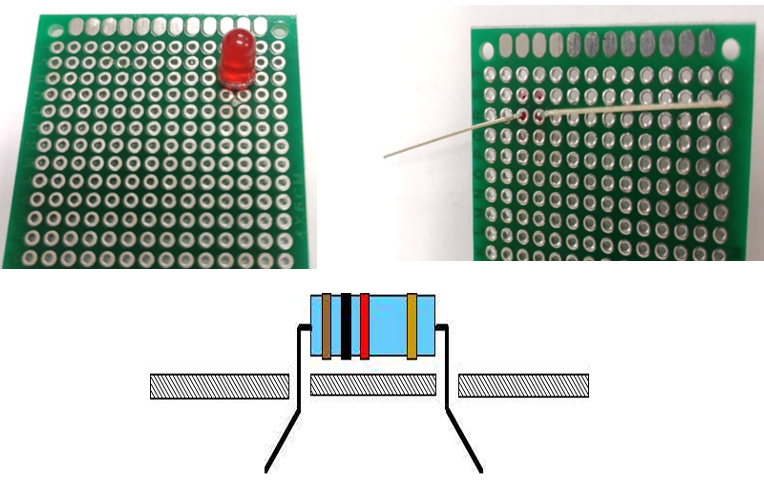
\includegraphics[scale=0.6]{EXP_00_Images/fig26.png}
\end{center}
\vspace{-8mm}
\begin{center} {Figure 26. Mounting the component on the PCB [7]}\end{center}

\noindent \textbf{Step 2: Apply Flux on the Hole and Heat the Joint  :}
First, apply the flux on the joint's hole and turn the soldering iron ON. At this point, touch the tip of the iron to the copper pad and the resistor lead simultaneously. We need to hold the soldering iron in place for 3-4 seconds to heat the pad and the lead.


\begin{center} 
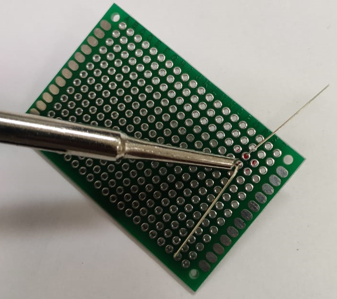
\includegraphics[scale=1]{EXP_00_Images/fig27.png}
\end{center}
\vspace{-8mm}
\begin{center} {Figure 27.Heat the joint}\end{center}


\noindent \textbf{Step 3: Apply Solder to Joint :}Continue holding the soldering iron on the copper pad and the lead and touch the solder to the joint. IMPORTANT : Don't touch the solder directly to the tip of the iron. We want the joint to be hot enough to melt the solder when it's touched. If the joint is too cold, it will form a bad connection.

\begin{center} 
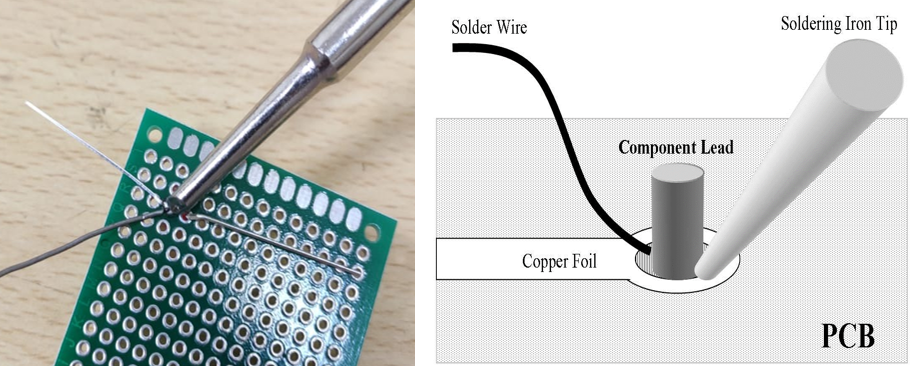
\includegraphics[scale=0.65]{EXP_00_Images/fig28.png}
\end{center}
\vspace{-8mm}
\begin{center} {Figure 28.Solder to joint [7]}\end{center}

\noindent \textbf{Step 4: Snip The Leads :}Remove the soldering iron and let the solder cool down naturally. Don't blow on the solder, as this will cause a bad joint. Once cool, we can snip the extra wire from leads. A proper solder joint is smooth, shiny, and looks like a volcano or cone shape. We want just enough solder to cover the entire joint but not too much, so it becomes a ball or spills to a nearby lead or joint.

\begin{center} 
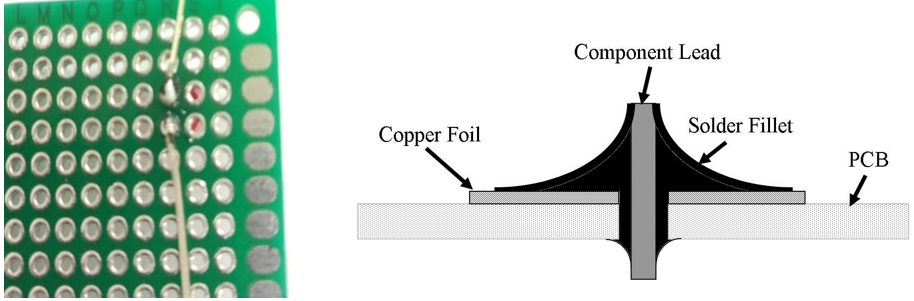
\includegraphics[scale=0.7]{EXP_00_Images/fig29.png}
\end{center}
\vspace{-8mm}
\begin{center} {Figure 29. Proper soldering [7]}\end{center}

\begin{center} 
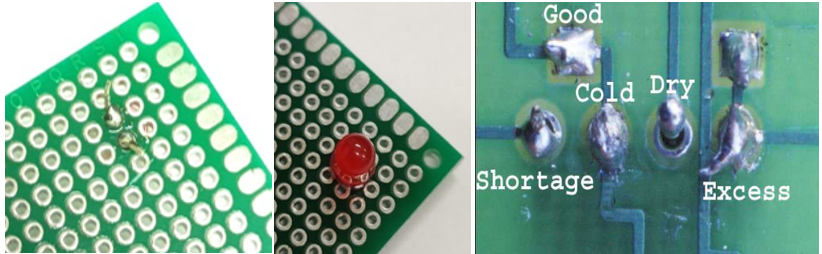
\includegraphics[scale=0.7]{EXP_00_Images/fig30.png}
\end{center}
\vspace{-8mm}
\begin{center} {Figure 30. Joint examples }\\
Watch this \href{https://www.youtube.com/watch?v=f95i88OSWB4&t=150s}{video} for the basics of soldering.
\end{center}

\begin{center} 
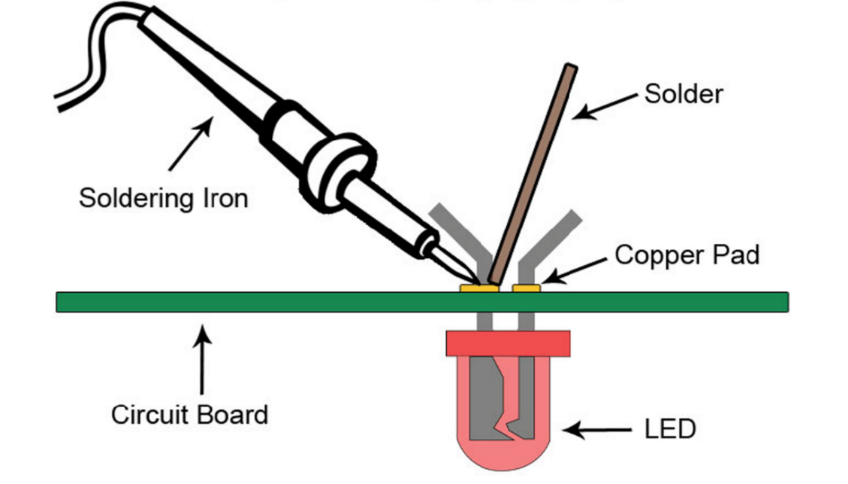
\includegraphics[scale=1.2]{EXP_00_Images/fig31.png}
\end{center}
\vspace{-8mm}
\begin{center} {Figure 31 Visualization of soldering an LED on a PCB [8] } \end{center}

\noindent \textbf{C. \underline{How to Solder Wire}}\\[6pt]
\textbf{Step 1:} Now it's time to show how to solder wires together. For this process, it's recommended to use helping hands or other types of clamp devices. Begin by removing the insulation from the ends of both wires we are soldering together. If the wire is stranded, twist the strands together with fingers.\\
\textbf{Step 2:} Ensure the soldering iron is fully heated and touch the tip to the end of one of the wires. Hold it on the wire for 3-4 seconds.\\
\textbf{Step 3:} Keep the iron in place and touch the solder to the wire until it's fully coated. Repeat this process on the other wire.\\
\textbf{Step 4:} Hold the two tinned wires on top of each other and touch the soldering iron to both wires. This process should melt the solder and coat both wires evenly.\\
\textbf{Step 5:}  Remove the soldering iron and wait a few seconds to let the soldered connection cool and harden. Use heat shrink to cover the connection.

\vspace{20mm}

\begin{center} {Table 4. Figures showing steps for soldering two wires [8]} \end{center}
\vspace{-8mm}
\begin{center} 
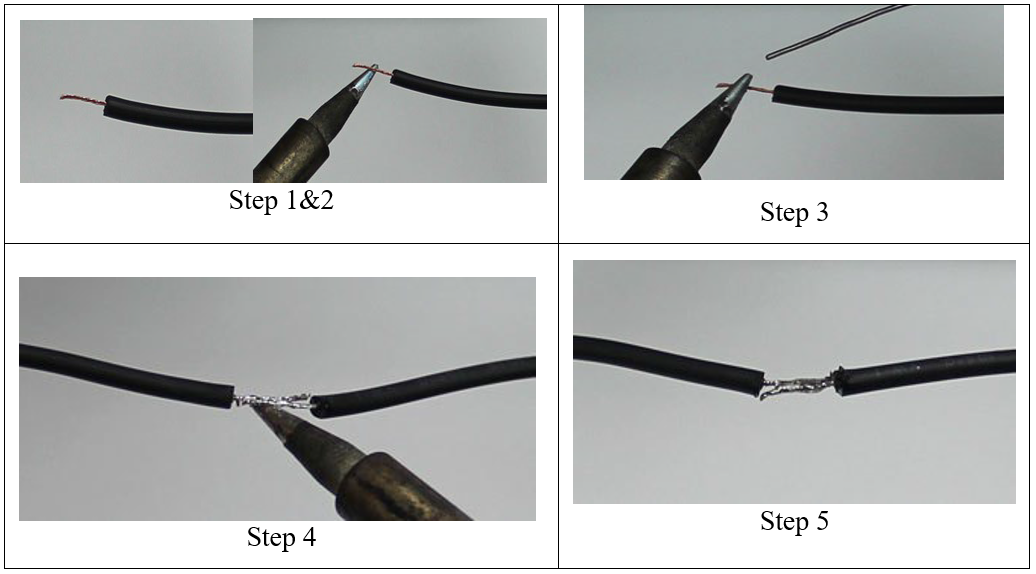
\includegraphics[scale=0.6]{EXP_00_Images/table4.png}
\end{center}



\noindent \textbf{D. \underline{How To Do Desoldering}}\\[6pt]
 The good thing about using solder is that it can be removed easily in a technique known as de-soldering. This thing comes in handy if we need to remove a component or correct the electronic circuit. To de-solder a joint, we will need solder wick, also known as a de-soldering braid.\\[6pt]
\textbf{Step 1:} Place a piece of the de-soldering braid on top of the joint/solder to be removed.\\
\textbf{Step 2:} Heat the soldering iron and touch the tip to the top of the braid. This process will heat the solder below, which will then be absorbed into the de-soldering braid. We can now remove the braid to see the solder has been extracted and removed. Be careful touching the braid when we are heating it because it will get hot.\\

\vspace{-8mm}
\begin{center} 
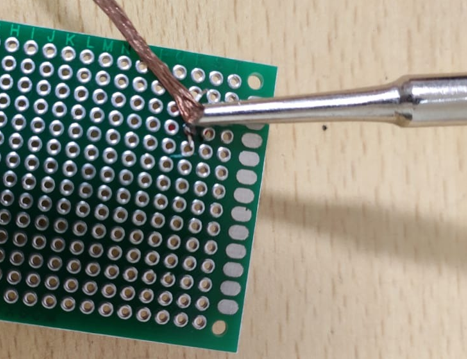
\includegraphics[scale=0.7]{EXP_00_Images/fig32.png}
\end{center}
\begin{center} {Figure 32. Desoldering} \end{center}

\noindent \textbf{Optional :}If we have many solders to be removed, we may use a device called a solder sucker. The solder sucker is a handheld mechanical vacuum that sucks up hot solder with a button press. To use, press the plunger down at the end of the solder sucker. Heat the joint with the soldering iron and place the tip of the solder sucker over the hot solder. Press the release button to suck up.

\vspace{4mm}
\noindent \textbf{\large REFERENCES:}
\vspace{-6mm}
\begin{enumerate}
\setlength\itemsep{-0.3em}


\item  \href{https://www.coolcircuit.com/how-to-use-a-multimeter-to-test-current}{Use-a-multimeter-to-test-current}
\item  \href{https://www.circuito.io/blog/breadboards}{Breadboards-II}
\item  \href{https://www.sciencebuddies.org/science-fair-projects/references/how-to-use-a-breadboard}{Breadboards-II}
\item  \href{http://wiring.org.co/learning/tutorials/breadboard}{Breadboards-III} 
\item  \href{http://wiring.org.co/learning/tutorials/diagrams/index.html}{Circuit diagrams}
\item  \href{https:/modelshop.co.uk/static/LEDs-resistors}{LEDs-resistors}
\item  \href{http://www.ece.ualberta.ca/~ee401/resource/manuals/Solder01.pdf}{Soldering}
\item  \href{https://www.makerspaces.com/wp-content/uploads/2017/04/How-To-Solder-Beginners-Guide.pdf}{How-To-Solder-Beginners-Guide.pdf }
\item  \href{https:/www.instructables.com/How-to-Use-a-Multimeter-Basics}{How-to-Use-a-Multimeter-Basics}
\item  \href{https://learn.sparkfun.com/tutorials/how-to-solder-through-hole-soldering/all}{ Through-Hole Soldering }
\item  \href{https://www.uts.edu.au/sites/default/files/Soldering_0.pdf}	{Soldering}


\end{enumerate}

\noindent \textbf{\large CONCEPT DRILLS:}
\vspace{-6mm}
\begin{enumerate}
 \setlength\itemsep{-0.3em}
\item Make a circuit by connecting two LEDs  and a Resistor in series 
\begin{enumerate}
 \setlength\itemsep{-0.3em}
\item	Measure voltages across the individual LED and Resistor and the voltage across the LED and Resistor in series
\item	Measure current going through the circuit.
\end{enumerate}
 
\item Make a soldering circuit in PCB with resistance, an LED, and later check with the power supply to see the glowing LED as shown below. Where Rx = 100 ohm
\end{enumerate}

\vspace{10cm}
\begin{center}
\noindent \textbf{APPENDIX}
\end{center}

\noindent \textbf{Resistor Color band Understanding}\\
Resistor values are often indicated with color codes. The chart below shows the numerical values of colors bands used to determine the resistance and tolerance for resistors.

\vspace{-4mm}

\begin{center} 
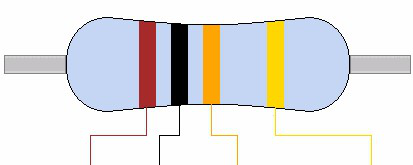
\includegraphics[scale=0.7]{EXP_00_Images/fig33_1.png}
\end{center}
\vspace{-8mm}
\begin{center} 
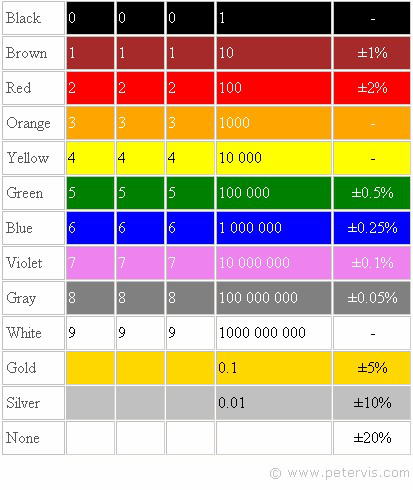
\includegraphics[scale=0.7]{EXP_00_Images/fig33_2.png}

{\href{https://www.petervis.com/electronics/Standard_Resistor_Values/10K.html} {Figure 33. Resistors color code and values}} \end{center}

\noindent \textbf{ Calculating resistance values for different color bands resistors}\\
\vspace{-4mm}
\begin{itemize}
\setlength\itemsep{-0.3em}
\item \textbf{4 band resistor:} These resistors have two bands for the resistance value (two significant digits), one multiplier, and one tolerance band.
\item \textbf{5 band resistor: }Resistors with high precision have an extra band to indicate a third significant digit. Therefore, the first three bands indicate the significant digits, the fourth band is the multiplication factor, and the fifth band represents the tolerance.
\item \textbf{6 band resistor: } These are used for high precision resistors that have an additional band to specify the temperature coefficient (ppm/˚C = ppm/K). The most common color for the sixth band is brown (100 ppm/˚C). This means that for a temperature change of 10 ˚C, the resistance value can change 1000 ppm = 0.1%.\\

\end{itemize}
\nonindent The table below shows the resistor value calculation examples for different color bands.

    

\begin{center} {\href{https://www.diyaudioandvideo.com/Electronics/ResistorColorCodes} { Table 5. Few examples of finding ohm value of different band resistors}} \end{center}
\begin{center}
\vspace{-4mm}
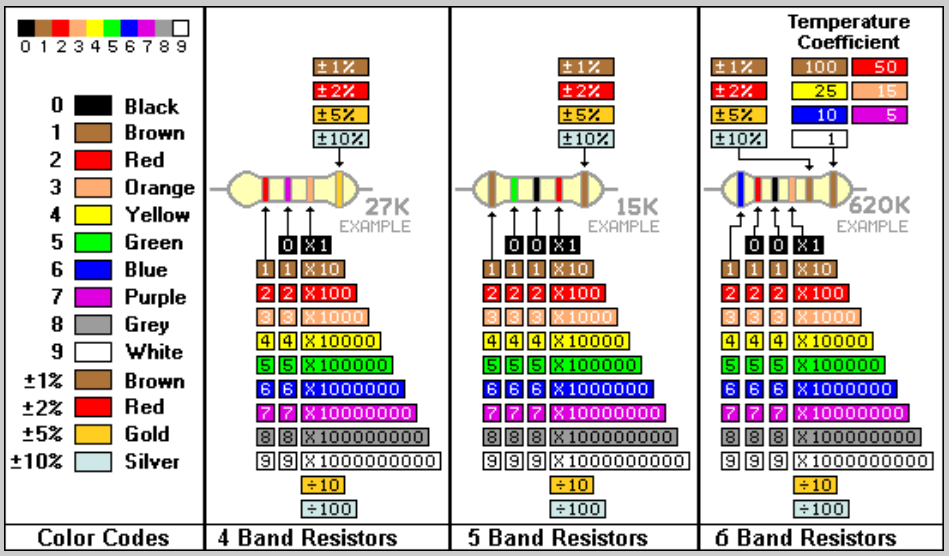
\includegraphics[scale=0.7]{EXP_00_Images/table5.png} \end{center}

\end{justify}
\end{document}